
%--------------------------------------------------------------------
%--------------------------------------------------------------------
% Formato para los talleres del curso de Métodos Computacionales
% Universidad de los Andes
%--------------------------------------------------------------------
%--------------------------------------------------------------------

\documentclass[11pt,letterpaper]{exam}
\usepackage{amsmath}
\usepackage[utf8]{inputenc}
\usepackage[spanish]{babel}
\usepackage{graphicx}
\usepackage{tabularx}
\usepackage[absolute]{textpos} % Para poner una imagen completa en la portada
\usepackage{hyperref}
\usepackage{float}

\newcommand{\base}[1]{\underline{\hspace{#1}}}
\boxedpoints
\pointname{ pt}

\extraheadheight{-0.15in}

\newcommand\upquote[1]{\textquotesingle#1\textquotesingle} % To fix straight quotes in verbatim



\begin{document}
\begin{center}
{\Large M\'etodos Computacionales} \\
Tarea 5 - \textsc{Markov Chain Monte Carlo}\\
13-11-2016\\
\end{center}

\begin{textblock*}{40mm}(10mm,20mm)
  
\includegraphics[width=3cm]{logoUniandes.png}
\end{textblock*}

\begin{textblock*}{40mm}(164mm,20mm)
  
\includegraphics[width=3cm]{logoUniandes.png}
\end{textblock*}

\vspace{0.3cm}


\noindent
La solución a este taller debe subirse por SICUA antes de las 8:00AM
del jueves 1 de diciembre del 2016. 

\noindent
Los c\'odigos deben encontrarse en un \'unico repositorio de \verb'github'
con el nombre \verb"NombreApellido_hw5". Por ejemplo yo deber\'ia
subir crear un repositorio con el nombre
\verb"JaimeForero_hw5". El \'ultimo commit de ese repositorio debe ser
anterior a las 8:00AM del jueves 1 de diciembre del 2016. 
Solamente se calificar\'an las tareas que tengan la direcci\'on 
del repositorio en sicuaplus.

\noindent
Adentro de ese repositorio deben existir tres
carpetas con los nombres \verb"punto_1", \verb"punto_2" y
\verb"punto_3" por cada uno de los puntos de esta tarea.  

\noindent
Dentro de cada carpeta deben estar los siguientes elementos.
\begin{itemize}
\item Un c\'odigo fuente en C que calcula las cadenas de Markov.
\item Un c\'odigo en Python que lee los datos producidos por el
  c\'odigo en C y produce visualizaciones de las densidades de
  probabilidad y los valores m\'as probables de los par\'ametros.
  Para esto deben utilizar la
  libreria \verb"corner"
  (\url{http://corner.readthedocs.io/en/latest/pages/quickstart.html}).
\item Un makefile que sique la estructura l\'ogica del punto para
  compilar y ejecutar el c\'odigo en C, ejecutar el codigo en Python y
  borrar todos los archivos auxiliares.   
\end{itemize}

\vspace{0.3cm}

\begin{questions}
\question{\bf{Lugar de un sismo}}
Una fuente s\'ismica se activo al tiempo $t=0$ en un lugar
desconocido de la superficie de la Tierra. Las ondas s\'ismicas
producida por la explosi\'on se grabaron por una red de seis
estaciones s\'ismicas ubicadas en las siguientes coordenadas (en km):
$(x_1,y_1)=(3,15)$,  $(x_2,y_2)=(4,15)$,  $(x_3,y_3)=(5,15)$,
$(x_4,y_4)=(3,16)$,  $(x_5,y_5)=(4,16)$,  $(x_6,y_6)=(5,16)$. Los
tiempos de llegada (en segundos) de las ondas s\'ismicas fueron 
$t_{obs,1}=3.12\pm\sigma_t$, $t_{obs,2}=2.98\pm\sigma_t$,
$t_{obs,3}=2.84\pm\sigma_t$, $t_{obs,4}=3.26\pm\sigma_t$,
$t_{obs,5}=3.12\pm\sigma_t$, $t_{obs,6}=2.98\pm\sigma_t$, donde
$\sigma_t=0.10$. 
\begin{itemize}
\item (10 puntos) Escriba un programa en C que implemente
  Metropolis-Hastings para
  encontrar la distribuci\'on de probabilidad de la posici\'on del
  epicentro dados los par\'ametros observacionales. Asuma que la
  Tierra es bidimensional y que la velocidad de propagaci\'on de las
  ondas es constante e igual a $5$ km/s.
\item (10 puntos)  Escriba un programa en Python que grafique la
  densidad de probabilidad en el plano $x,y$ y 
  muestre los valores m\'as probables junto a sus
  incertidumbres. 
\item (5 puntos) Escriba un \verb"makefile" que enlace correctamente
  todos los pasos anteriores.

\end{itemize}

\question{{\bf Ley de gravitaci\'on}}
Los siguientes datos (tomados de este art\'iculo
\url{https://arxiv.org/abs/0903.5308}) muestran la velocidad y
posici\'on instant\'anea de los planetas en el sistema solar para el
primero de abril del 2009.

\begin{figure}[H]
  \centering
  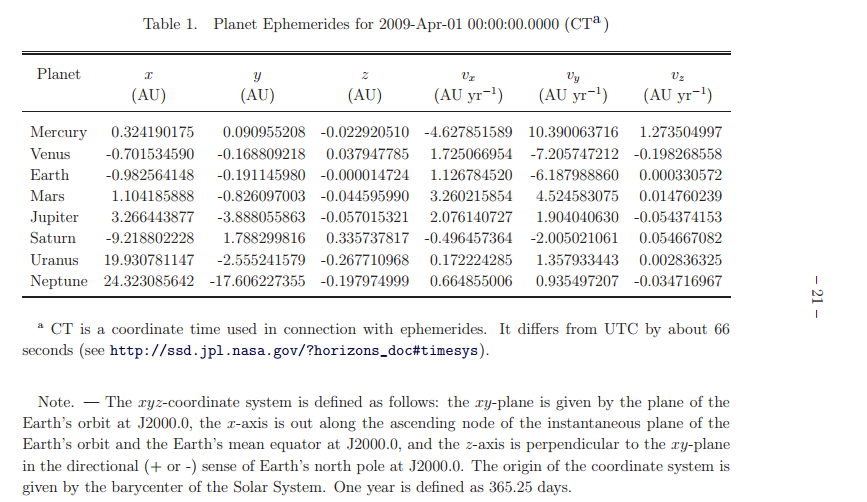
\includegraphics[width=18cm]{planetas}
  \caption{\label{fig:gridplates} Posiciones y velocidades
    instant\'aneas de planetas con respecto al Sol .}
\end{figure}

\begin{itemize}
\item (10 puntos) Escriba un programa en C que implemente
  Metropolis-Hastings para encontrar la distribuci\'on de probabilidad
  del logaritmo de la masa del Sol y del exponente que describe como
  escala la acelaraci\'on radial en funci\'on de la distancia al
  Sol. Asuma que las \'orbitas de los planetas son perfectamente
  circulares. 
\item (10 puntos) Escriba un programa en Python que grafique la
  densidad de probabilidad en el plano $\log_{10} M_{sol},\alpha$ y 
  muestre los valores m\'as probables junto a sus
  incertidumbres. 
\item (5 puntos) Escriba un \verb"makefile" que enlace correctamente
  todos los pasos anteriores.
\end{itemize}


\question{{\bf Poblaciones}}
Un grupo de bi\'ologos toma datos por casi una d\'ecada de una
poblaci\'on de presas y predadores. Los bi\'ologos intuyen que el
n\'umero de presas $x$ y el numero de predadores $y$ se describe por
un modelo del tipo Lotka-Volterra con las siguientes ecuaciones:

\begin{equation}
\frac{dx}{dt}=x(\alpha - \beta y),
\end{equation}
\begin{equation}
\frac{dy}{dt}=-y(\gamma -\delta x).
\end{equation}

donde $\alpha$, $\beta$, $\gamma$ y $\delta$ son par\'ametors libres
que se quieren buscar a partir de los datos experimentales.

\begin{itemize}
\item (30 puntos) Escriba un programa en C que implemente
  Metropolis-Hastings para
  encontrar la distribuci\'on de probabilidad de los par\'ametros
  dados los datos observacionales.
  \verb"lotka_volterra_obs.dat"\footnote{El archivo se encuentra en
\url{https://github.com/ComputoCienciasUniandes/MetodosComputacionalesDatos/blob/master/homework/2016-20/hw5/lotka_volterra_obs.dat}}.

\item (15 puntos) Escriba un programa en Python que grafique la
  densidad de probabilidad de los par\'ametros y 
  muestre los valores m\'as probables de junto a sus
  incertidumbres. 

\item (5 puntos) Escriba un \verb"makefile" que enlace correctamente
  todos los pasos anteriores.
\end{itemize}


\end{questions}

\end{document}

